\section{Background}

In this section we briefly introduce the key definitions and the necessary parsing algorithm. Before descibing the Valiant's  algorithm, we would like to mention one of the basic recognition algorithms known as CYK (the Cocke-Younger-Kasami algorithm), by which we show the main Valiant's idea that made such time complexity possible.

\subsection{Preliminaries}

An alphabet $\Sigma$ is a finite nonempty set of symbols. $\Sigma^{*}$ is a set of all finite strings over $\Sigma$.
A grammar is a quadruple $(\Sigma, N, R, S)$, where $\Sigma$ is a finite set of terminals, N is a finite set of nonterminals, R is a finite set of productions of the form $\alpha \rightarrow \gamma$, where $\alpha \in V^{*}NV^{*}$, $\gamma \in V^{*}$, $V = \Sigma \cup N$ and $S \in N$ is a start symbol.

\subsubsection{Definition 1} Grammar $G = (\Sigma, N, R, S)$ is called context-free, if $\space\forall r \in R$ are of the form $A \rightarrow \beta$, where $A \in N, \beta \in V^{+}$.

\subsubsection{Definition 2} Context-free grammar $G = (\Sigma, N, R, S)$ is said to be in Chomsky normal form if $\space\forall r \in R$ are of the form:
\begin{itemize}
  \item $A \rightarrow BC$,
  \item $A \rightarrow a$,
  \item $S \rightarrow \epsilon$,
\end{itemize}
where $A, B, C \in N, a \in \Sigma, \epsilon$ is an empty string.

\subsubsection{Definition 3} $L_{G}(A)$ is language of grammar $G_{A} = (\Sigma, N, R, A)$, which means all the sentences that can be derived in a finite number of rule applications from the start symbol A.

\subsection{Parsing by matrix multiplication}

The main problem of parsing is to verify if the input string belongs to the language of some given grammar $G$. We will describe the Cocke-Younger-Kasami algorithm and the most asymptotically efficient parsing algorithm, which works for all context-free grammars, Valiant's parsing algorithm, based on matrix multiplication. In this paper we use the rewritten version of Valiant's algorithm proposed by Alexander Okhotin.

The CYK algorithm is a basic parsing algorithm. Its main idea is to construct for an input string $a_{1}a_{2}...a_{n}$ a parsing table T of size $n \times n$,  where
\begin{equation}
T_{i, j} =  \{ A |  a_{i + 1}...a_{j} \in L_{G}(A)\} \quad \forall i < j
\end{equation}
and $G = (\Sigma, N, R, S)$ is a context-free grammar in Chomsky normal form.

The elements of T are filled successively beginning with
\begin{equation}
T_{i - 1, i} = \{ A | A \rightarrow a_{i} \in R\}
\end{equation}
Then,
\begin{equation}
T_{i, j} = f(P_{i, j})
\end{equation}
where
\begin{equation}
P_{i, j} = \bigcup\limits_{k = i + 1}^{j - 1} T_{i,k} \times T_{k, j}
\end{equation}
\begin{equation}
f(P) = \{A | \exists A \rightarrow BC \in R : (B, C) \in P\}
\end{equation}

The input string $a_{1}a_{2}...a_{n}$ belongs to $L_{G}$ if and only if $S \in T_{0, n}$.

% Algorithm1
\begin{algorithm}
\SetAlgoNoLine
\KwIn{Grammar $G = (\Sigma, N, R, S), w = a_{1}...a_{n}, n \geq 1, a_{i} \in \Sigma$, where  n + 1 --- power of two}
\underline{main()}{:}{

 \textit{compute(0, n + 1)\;}
 accept if and only if $S \in T_{0, n}$
 \linebreak
 }

\underline{compute(\textit{l, m})}{:}{

 \If {$m - l \geq 4$}{
     \textit{compute(l, $\frac{l+m}{2}$)\;
     compute($\frac{l+m}{2}$, m)}}
 \textit{complete(l, $\frac{l+m}{2}$, $\frac{l+m}{2}$, m)}
 \linebreak
 }

\underline{complete(\textit{l, m}, $l^\prime$, $m^\prime$)}{:}{

 \If {$m - l = 4$ and $m = l^\prime$}{$T_{l, l + 1} = \{A | A \rightarrow a_{l+ 1} \in R\}$\;}
 \ElseIf{$m - l = 1$ and $m < l^\prime$}{ $T_{l, l'} = f(P_{l, l'})$\;}
 \ElseIf{$m - l > 1$}{
    $leftgrounded = (l, \frac{l+m}{2}, \frac{l+m}{2}, m), rightgrounded = (l', \frac{l'+m'}{2}, \frac{l'+m'}{2}, m')$,

    $bottom = (\frac{l+m}{2}, m, l', \frac{l'+m'}{2}), left = (l, \frac{l+m}{2}, l', \frac{l'+m'}{2})$,

    $right = (\frac{l+m}{2}, m, \frac{l'+m'}{2}, m'), top = (l, \frac{l+m}{2}, \frac{l'+m'}{2}, m')$\;
    complete(bottom)\;
    $P_{left} = P_{left} \cup (T_{leftgrounded} \times T_{bottom})$\;
    complete(left)\;
    $P_{right} = P_{right} \cup (T_{bottom} \times T_{rightgrounded})$\;
    complete(right)\;
    $P_{top} = P_{top} \cup (T_{leftgrounded} \times T_{right})$\;
    $P_{top} = P_{top} \cup (T_{left} \times T_{rightgrounded})$\;
    complete(top)
    }
 }
\caption{Parsing by matrix multiplication: Valiant's Version}
\end{algorithm}

The time complexity of this algorithm is $O(n^3)$. Valiant proposed to offload the most intensive computations to the Boolean matrix multiplication. As the most time-consuming is computing $\bigcup\limits_{k = i + 1}^{j - 1} T_{i, k} \times T_{k, j}$, Valiant rearranged computation of $T_{i, j}$, in order to use multiplication of submatrices of T.

\subsubsection{Definition 4} Let $X \in (2^N)^{m \times l}$ and $Y \in (2^N)^{l \times n}$ be two submatrices of parsing table T. Then, $X \times Y = Z$, where $Z \in (2^{N \times N})^{m \times n}$ and $Z_{i, j} = \bigcup\limits_{k = 1}^{l} X_{i, k} \times Y_{k, j}$.

In \textbf{Algorithm 1} full pseudo-code of Valiant's algorithm is written in the terms proposed by Okhotin, is presented. All elements of T and P are initialized by empty sets. Then, the elements of these two table are successively filled by two recursive procedures.

The procedure $compute(l, m)$ constructs the correct values of $T_{i,j} \forall l \le i < j < m$.

The procedure $complete(l, m, l', m')$ constructs the submatrix $\forall T_{i, j}$ $l \le i < m$, $l' \le j < m'$. This procedure assumes $T_{i, j} \forall l \leq i < j < m,  l' \leq i < j < m'$ are already constructed and the current value of  $P[i, j] =  \{ (B, C) |\exists (m \le k < l'): a_{i + 1}...a_{k} \in L(B), a_{k + 1}...a_{j} \in L(C)\}$ $\forall l \leq i < m,  l' \leq j < m'$. \textbf{Figure 1} shows how the submatrix division during the procedure call is happening.

\begin{figure}[h]
\centering
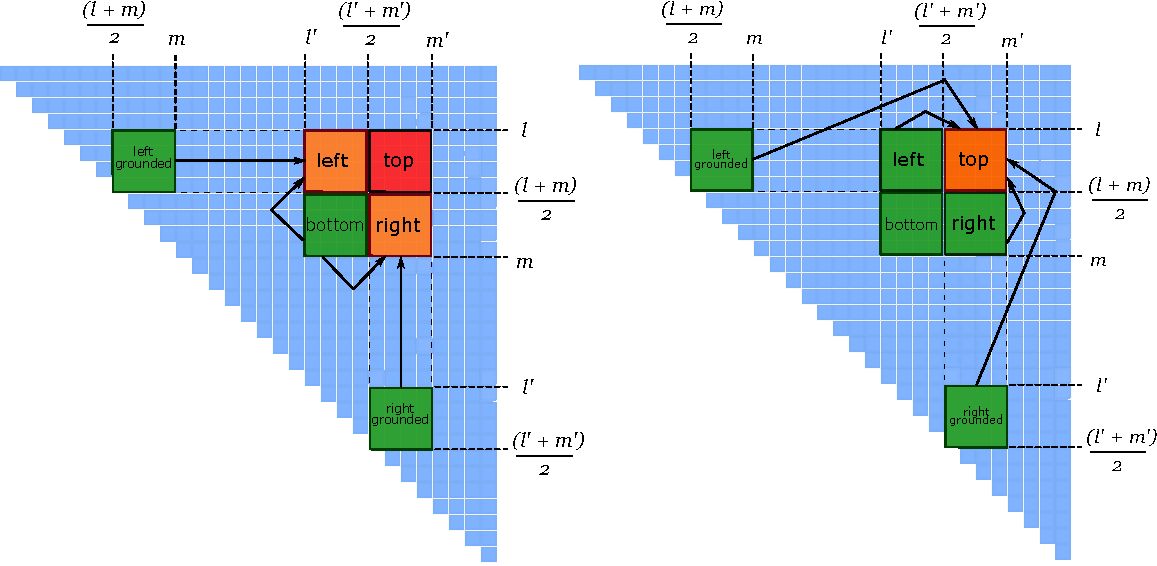
\includegraphics[width=200pt]{splitting.pdf}
\centering
\caption{Matrix partition used in $complete(l, m, l', m')$ procedure} \label{fig1}
\end{figure}

Then Valiant described that product of multiplying of two submatrices of parsing table T can be provided as $|N|^2$ Boolean matrices (for each pair of nonterminals). Denote matrix corresponding to pair $(B, C) \in N \times N$ as $Z^{(B, C)}$, then $Z_{i, j}^{(B, C)} = 1$ if and only if $(B, C) \in Z_{i, j}$. It should also be noted that $Z^{(B, C)} = X^{B} \times Y^{C}$. So, matrix multiplication in \textbf{Definition 4} can be replaced by Boolean matrix multiplication, each of which can be computed independently. Following these changes, time complexity of \textbf{Algorithm 1} is $O(|G|BMM(n)log(n))$ for an input string of length n, where BMM(n) is the number of operations needed to multiply two Boolean matrices of size $n \times n$.
